\chapter{Background}

\section{Power Systems and Frequency}
Interconnected power systems are comprised of power generating units and energy storage systems connected to transmission and distribution networks. Generated power is used to service load demand. A single line diagram of a power network can be seen in Figure \ref{fig:generation}. The diagram shows how thermal generation units (left-hand side), such as coal and nuclear, in addition to renewable sources of generation, like wind and solar provide a power generation mix that is transmitted by a network for the consumers of generated energy: industry and households (right-hand side).
\begin{figure}[ht]
	\centering
	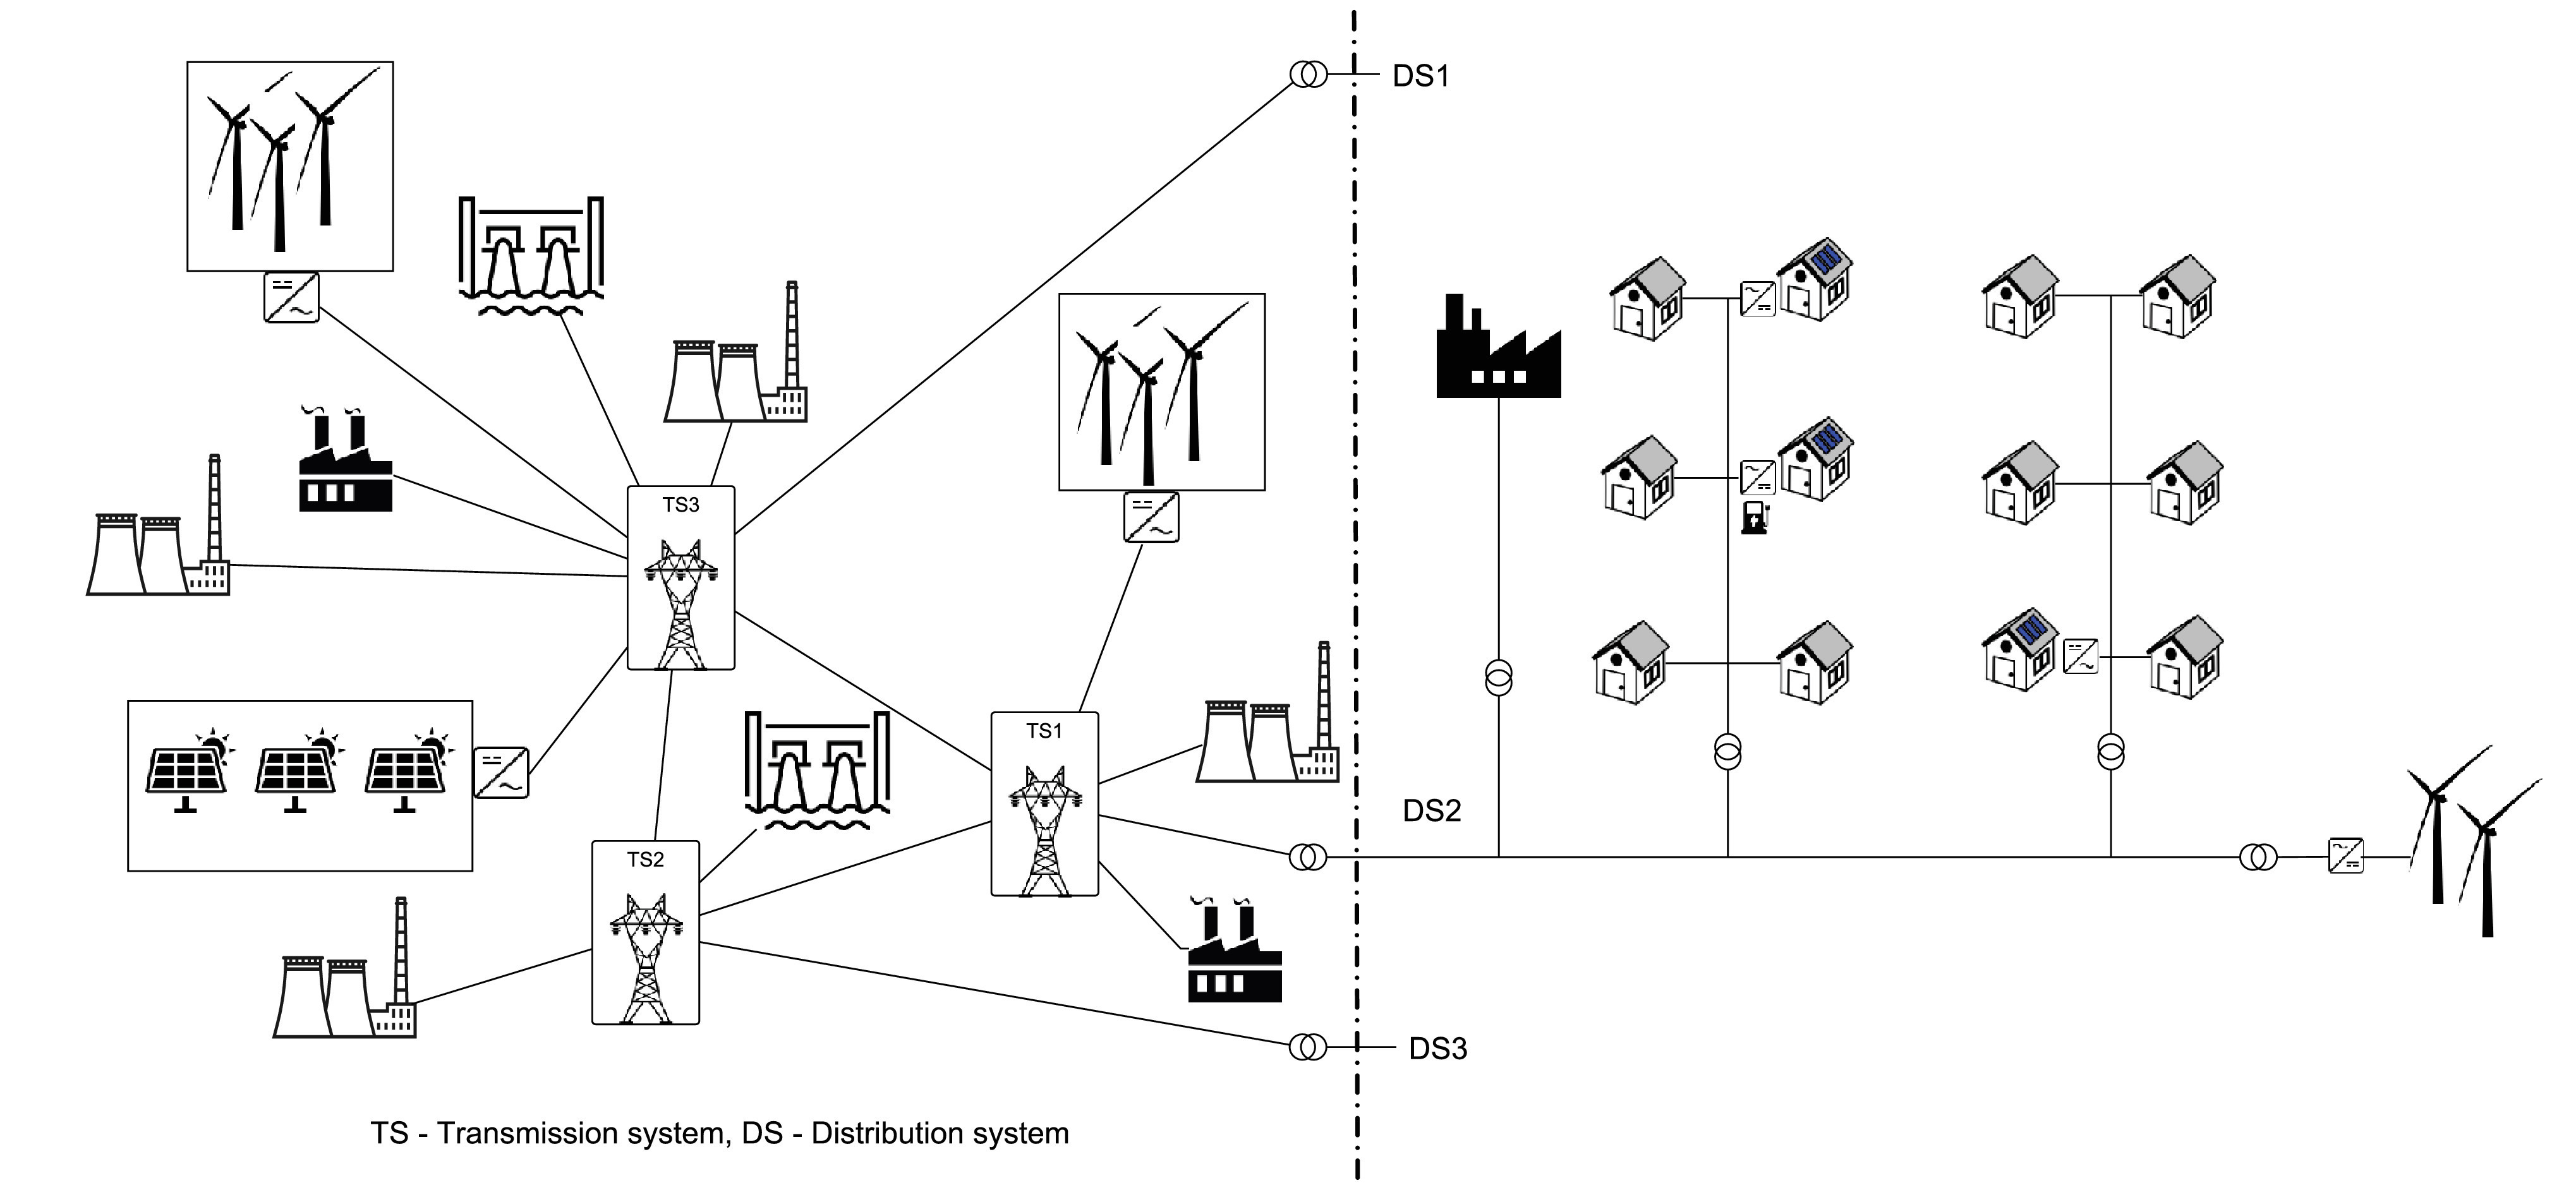
\includegraphics[scale=0.85]{power_system}
	\caption{A single line diagram of a typical power system. The image shows points of generation from thermal and renewable sources, and the subsequent supply of generated energy to meet load demand through the transmission and distribution network \cite{Glavic2019}.}
	\label{fig:generation}
\end{figure}

One of the key elements to successful operation of interconnected power systems is ensuring total load demand is matched with total generation while taking into account power losses involved with generation, transmission, and distribution \cite{Wood2013}. To understand why it is important to match generation with load demand consider the basic operation of a single thermal generator. 
\begin{figure}[h]
	\centering
	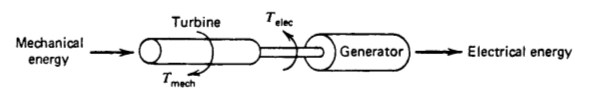
\includegraphics[height=1.4cm]{generation}
	\caption{A thermal generation unit consisting of a prime mover (turbine), and a synchronous machine \cite{Wood2013}.}
	\label{fig:turbine}
\end{figure}

The essential elements of a thermal generator are a prime mover (such as a gas turbine) and a synchronous machine, as depicted in Figure \ref{fig:turbine}. The prime mover provides mechanical torque, $T_{mech}$, which drives the synchronous machine producing electrical energy. In response, the synchronous machine creates an opposing torque that depends on the size of the load demand. This opposing torque is referred to as electrical torque and is denoted as $T_{elec}$. If $\alpha$ represents angular acceleration of the generator rotating mass, and $I$ is its moment of inertia, then by Newton's second law:
\begin{equation}
	T_{mech} - T_{elec} = I \alpha \label{eq:1}
\end{equation}

When $T_{mech}$ equals $T_{elec}$ the system will be in a steady state of zero angular acceleration with a constant angular velocity, $\omega$. Now, if $T_{mech} > T_{elec}$, then the system has an angular acceleration causing the angular velocity, $\omega$, to increase. This results in a frequency increase in the system. Conversely, if $T_{mech} < T_{elec}$ then the angular velocity $\omega$ will decrease, resulting in a frequency decrease. It is important to note that, at any point in time, the total electrical load demand will fluctuate as businesses and households switch grid connected appliances or motors on and off. The result is that an uncontrolled system will have a continually changing frequency. Australia's electricity network is designed to operate at a frequency of 50$\si{\hertz}$. In the majority of network scenarios, the Australian Energy Market Operator (AEMO) has a desired operating range for frequency which lies between 49.85 and 50.15$\si{\hertz}$ \cite{AEMOfreqdev}. Similarly, the Power and Water Corporation (PWC) network technical code for the Northern Territory states that under normal operating conditions frequency should be maintained in the range of 49.80 to 50.20$\si{\hertz}$ \cite{Pwc2013}. Network operation outside of the specified range can cause damage to electrical equipment such as transformers or motors, which are designed to operate at specific frequencies \cite{Sen2014}. Network designers engineer protection schemes so that sustained frequency excursions outside of the allowed range will cause equipment to trip from the network \cite{AEMOpowerfreqriskrev}.

\begin{figure}[ht]
	\centering
	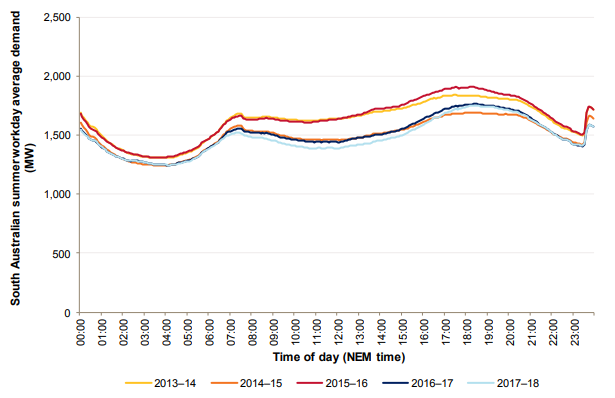
\includegraphics[height=7cm]{load_profile}
	\caption{Weekday energy demand profile in South Australia during summer \cite{Aemosaenergyrep}.}
	\label{fig:energydemand}
\end{figure}

\newpage

Protection schemes tripping equipment from the network is undesirable as this can leave households and industry without power, resulting in economic loss. Further, if disconnections are uncontrolled the system stability is reduced \cite{AEMOpowerfreqriskrev}. System controllers, such as the AEMO and PWC, are interested in being able to control the system to follow changes in load demand so that system frequency is maintained in the allowable range. Additionally, they are interested in control mechanisms to restore frequency excursions as a result of unexpected disturbances. System controllers can use historical data, like that shown in Figure \ref{fig:energydemand}, to forecast daily demand profiles with some reliability. This type of forecasting does not help when trying to predict the occurrence of random disturbances; however, it does provide a starting point for estimating required generation needed to meet demand. It is important to note that forecasting is not perfect. Inevitably mismatches in supply and demand will occur causing small imbalances between $T_{mech}$ and $T_{elec}$, resulting in a change to angular velocity $\omega$ and the network frequency \cite{Glover2012}. To perfectly match supply and demand, system controllers use generators referred to as regulating units, placed under Automatic Generation Control (AGC) \cite{Kothari2011}. A regulating unit is a generator that has the capacity to increase or decrease mechanical torque $T_{mech}$, and AGC is the name used for a system providing control over the mechanical torque output of regulating generators. If the system controller has a sufficient number of regulating units under AGC it can perform two functions: load following, and restoring the system to stable operating conditions in the event of a disturbance \cite{Grainger1994}. Using a regulating unit under AGC control to load follow is referred to, by AEMO, as load following ancillary services \cite{AEMOancilliaryserv}.

\begin{figure}[ht]
\centering
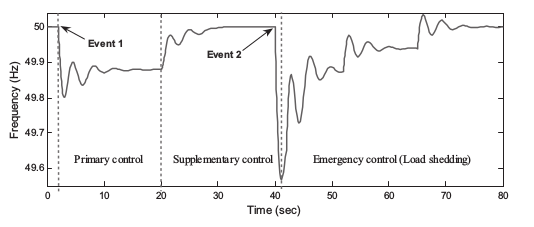
\includegraphics[height=6cm]{frequency_arrest}
\caption{A minor frequency disturbance occurs at the 2 sec mark and primary control systems (governors) arrest the frequency drop. System frequency is adjusted to desired 50$\si{\hertz}$ operating level using AGC control of regulating units. This referred to as supplementary (or secondary) control in the literature. AEMO refers to this as load following ancilliary services. At the 40 sec mark the network experiences a major frequency disturbance which is arrested by emergency control measures such as under-frequency load shedding (UFLS). System restoration is aided using AGC control of regulating units, which AEMO refers to as spinning reserve ancillary services \cite{Bevrani2011}.}
\label{fig:freqarrest}
\end{figure}

\newpage

Load following control adjusts regulating units in order to match supply with a demand load profile, and maintain frequency in a normal operating range a shown in the first 40 seconds of Figure \ref{fig:freqarrest}. Using a regulator under AGC control to restore the system after a major disturbance is referred to, by AEMO, as providing spinning reserve ancillary services. \cite{AEMOancilliaryserv}. When used in either fashion it is important to note that the regulating unit is not responsible for arresting frequency excursions, rather, it is used to restore the system back to the allowable frequency operating range after the frequency excursion has been arrested. An example of a frequency excursion, arrest, and subsequent restoration for minor and major disturbances can be seen in Figure \ref{fig:freqarrest}. AEMO and PWC do not require all generators on the network to act as regulating units since adequate frequency control can be achieved using a subset of the total available generators.


\subsection{Frequency Control for a Single Area System}\label{oneareapowersystem}
The power system model shown in Figure \ref{fig:energyts} depicts total generation coming from many generation assets --- this is complex to model. Researchers often find it useful to divide generation assets into sub-groups referred to as control areas \cite{Kothari2011}. A control area is defined as a subset of generators that are in close proximity to each other and constitute a coherent group that speed up and slow down together, maintaining their relative power angles \cite{Kothari2011}. Therefore, the total network is comprised of many interconnected control areas. An example of this can be seen in Figure \ref{fig:interconnectedpa}. Notice that for each area there is only one load and one generator.
\begin{figure}[ht]
	\centering
	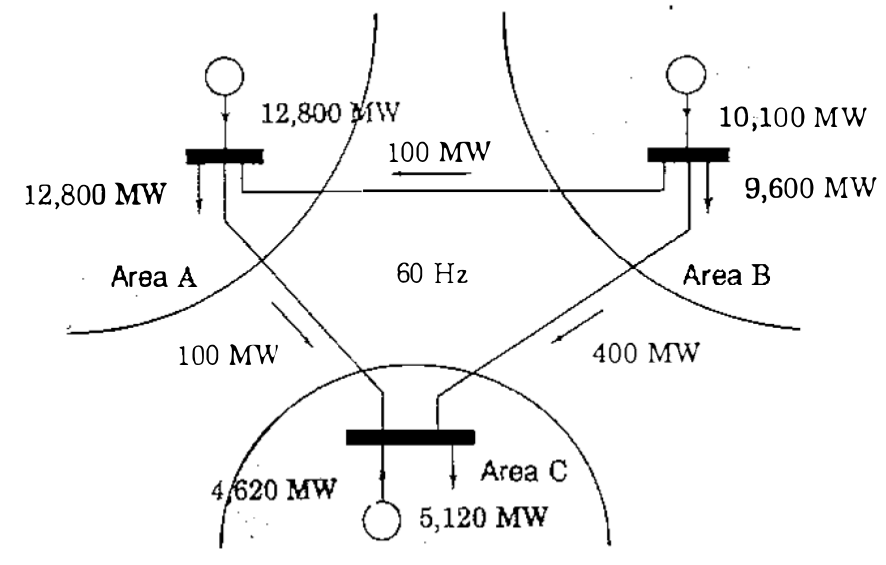
\includegraphics[height=8cm]{multiple_area_system}
	\caption{An example of three interconnected control areas in a 60$\si{\hertz}$ power system. The interconnections allow power to flow from one area to another, allowing generators to service loads from different areas. Each control area consists of several generators and loads, but are modelled with a single generator and single load for simplicity \cite{Grainger1994}.}
	\label{fig:interconnectedpa}
\end{figure}

Typically, for each control area, researchers will aggregate many loads into a single load, and many generators into a single generator. This simplifies the model further \cite{Grainger1994}. The simplest power system to control is one that consists of a single control area. A single control area power system has no interconnections to any other control area. It is comprised of a consumer load demand, and a set of generators, some of which are acting as regulating units. As previously mentioned, for modelling simplicity, loads are aggregated to a single load, and generators can be aggregated to a single generator. This simple system is well understood. It is generally acknowledged that a speed droop governor feedback control regime will perform primary frequency control, and an AGC feedback loop is used to perform secondary frequency control when restoring a minor frequency excursion \cite{Wood2013, Grainger1994, Kothari2011, Kundur1994}. A particularly well laid out approach to developing linear models for the turbine, generator, load, and governor was presented by Kundur \cite{Kundur1994}. The full model is shown in Figure \ref{fig:singleareacontrol}. This particular model provides generator models for regulating and non-regulating generators. The governor blocks are first-order linear models of the speed governors. The turbine blocks are first-order models of the turbines. The final block is the generator load, which is also a first order system. The AGC feedback loop uses an integral controller.

\begin{figure}[ht]
\centering
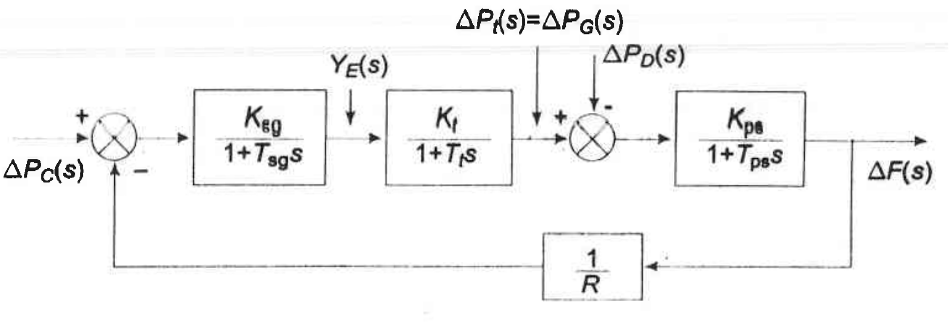
\includegraphics[height=8cm]{single_area_control}
\caption{A classical feedback control approach for a single control area power system. The system is comprised of a first order models for both turbines, and generators. The governor controllers are also first order models. AGC is implemented using an integral control block in a feedback loop \cite{Kundur1994}.}
\label{fig:singleareacontrol}
\end{figure}

\newpage

\subsection{Frequency Control for Two Area System}
The single area system presented in Section \ref{oneareapowersystem} is useful to help understand the role of governors and AGC in controlling power system frequency. In reality, power systems are comprised of many control areas connected by transmission lines (referred to in the literature as tie lines). Often it is the case that there is some net power transfer over the tie lines, enforceable by economic contract. Single area models do not provide for this additional complexity.

\begin{figure}[ht]
	\centering
	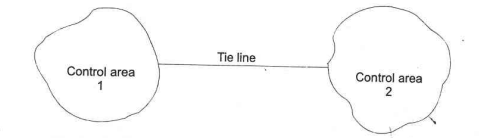
\includegraphics[height=3cm]{two_area_system}
	\caption{A two area power system comprised of generators and load connected via a tie line. Power flows from one area to the other depending on the power demands.}
	\label{fig:twoareapower}
\end{figure}

Distinct control areas are typically thought of as different participants in the generation market, or simply as different regions in which generation assets are based \cite{Kothari2011}.

\begin{figure}[ht]
	\centering
	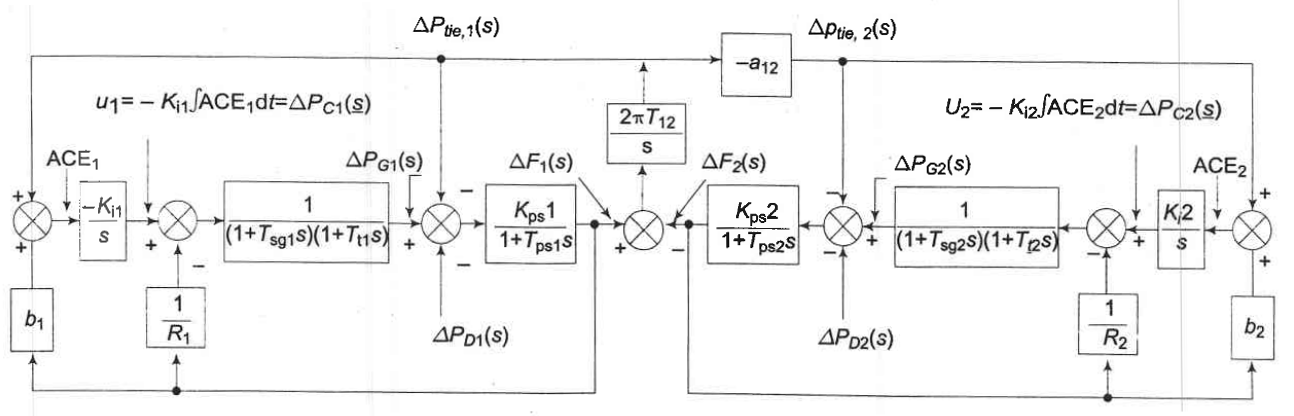
\includegraphics[height=12cm]{two_area_control_block}
	\caption{A classical feedback control approach to a two area power system \cite{Kundur1994}.}
	\label{fig:twoareacontrolblock}
\end{figure}

The simplest model that includes tie lines is the two area power system, shown in Figure \ref{fig:twoareapower}. The control objective with this system is to maintain the inter-area power transfer, whilst regulating the frequency of each area. An AGC integral feedback loop on regulating units, like that shown in Figure \ref{fig:singleareacontrol}, would ensure that power system frequency is maintained, however, would not guarantee inter-area power transfer agreements are observed. Violation of power transfer contracts due to control issues does not allow for a stable market in which energy can be reliably traded. Fortunately, multi control area power systems are well understood. Linear models have been developed to simulate these systems, and classical control approaches have been successfully implemented to meet the new control objectives. In order to achieve this, a metric called Area Control Error (ACE) is used in the AGC feedback loop for each control area. ACE is a linear combination of the frequency deviations and the . The implementation of this control system is shown in Figure \ref{fig:twoareacontrolblock}.

% % % % % % % % % % % % % % % % % % % % % %

\section{Reinforcement Learning}\label{rl}
According to Sutton and Barto's seminal text \cite{Sutton2018}, reinforcement learning (RL) is a branch of machine learning, based on trial-and-error, that is concerned with sequential decision making. An RL agent exists in an environment where it can act and receive a reward. The environment is modelled as a set of probabilistic transitions between states, for a set of possible actions that can be selected by the agent. A state transition presents the agent with a reward signal that informs the agent whether an action taken was good or bad. This environmental architecture is referred to as a Markov Decision Process (MDP). It is the agent's objective to maximise the reward it will receive in the future. An agent can achieve this by learning an optimal policy which maps environment states to actions. Learning such a policy is key idea in RL, and the agent achieves this by experimentation.

\subsection{Markov Decision Process}
Bellman's pioneering work on the Markov Decision Process (MPD) provided the necessary architecture to develop RL algorithms \cite{Bellm1957}. His work considered an agent that exists in some environment comprised of many discrete states, $s \in S$, such that $S$ denotes the state space. At any discrete point in time the agent can take action $a \in A$, where $A$ denotes the action space. When the agent takes an action in a given state, the agent receives some reward, denoted with $r \in R$, where $R$ is the set of rewards. Fundamental to Bellman's MDPs were the state transition dynamics which were defined by probabilities: if an agent is in a given state, $s$, and takes action, $a$, this will transition the agent to a new state, $s'$, and yield reward, $r$, with some given probability. This set of probabilities are referred to as the state transition probabilities, and are denoted as follows:

\begin{equation}
	P(S_{t+1} = s', \ R_{t+1} = r | S_t = s, \ A_t = a) = p(s', r | s, a) \label{eq:21}
\end{equation}

The set of parameters outlined above, and expression \ref{eq:21}, make up a framework referred to as an MDP.

\subsection{Returns, Episodes, and Policy} \label{rep}
In addition to  developing the MDP framework, Bellman was also responsible for key developments in a field of research called dynamic programming (DP) \cite{Bellm1954}. Assuming that the agent has complete knowledge of the state transition probabilities of an environment, DP algorithms can be used to determine analytical solutions for the problem of how an agent should behave to maximise it's cumulative reward \cite{Bellm1954, Howard1960}. This idea is distinct from RL but was critical in RL's development. DP provides the agent with complete knowledge of it's environment, whereas the RL agent has no knowledge of the environment dynamics and must learn as well as how to maximise it's cumulative reward \cite{Sutton2018}. Many researchers made links between DP and RL \cite{Bellm1959, Witten1977, Werbos1987}, but it wasn't until 1989 that Watkins presented the first formal treatment of RL in an MDP framework, paving the way for modification of DP algorithms for use with RL problems \cite{Watkins1989}. Three of the central ideas used in DP algorithms are episodes, returns, and policies \cite{Sutton2018}.

The duration of time that an agent will spend taking actions and transitioning states before encountering a terminal state is defined as an episode. It is the agent's goal to take actions such that it maximises the sum of all the rewards as it concludes an episode. The cumulative sum of rewards is called the return. Consider an agent taking an action at each discrete time step, $t$, and receiving reward, $r_t$, after each action. If there are $N$ discrete time steps before the agent reaches a terminal state, Bellman defines the return as:

\begin{equation}
	G_t = \sum_{k = 0}^{N-1} r_{t + k} \label{eq:22}
\end{equation}

Rewards received in the future are often perceived as less valuable than rewards received in the present. To account for this Bellman used a discount factor applied to each reward in the sequence. Letting $\gamma \in [0,1]$ then \ref{eq:22} becomes:

\begin{equation}
	G_t = \sum_{min}^{max}\gamma^k r_{t+k} \label{eq:23}
\end{equation}

Finally, in order for the agent to take actions it must have a belief of what action it should take, given it's current state. This belief is called a policy and denoted as $\pi$ \cite{Sutton2018}. Sutton and Barto define a  policy as the mapping of states to actions i.e. a rule that determines what actions the agent should take for a given state. A policy can be deterministic, and depend only on the state, $\pi(s)$, or stochastic, $\pi(a|s)$, such that it defines a probability distribution over the actions, for a given state. An optimal policy, denoted $\pi*$, is a policy which will maximise the return an agent receives over an episode.

\subsection{Value Function and the Bellman Equations}
The basic principal of dynamic programming is to assign a value to each state that informs an agent how useful a state is to achieving a high cumulative reward. Watkins refers to the creation of systems that assign values to state as solving the credit assignment problem \cite{Watkin1989}. Bellman's approach to solving credit assignment was to develop functions that assigned values to states \cite{Bellm1954}. Bellman's value function, $V_{\pi}(s)$ , is defined as the expected sum of the discounted return, $G_t$, that the agent will receive while following policy $\pi$ from a particular state $s$. Mathematically, this is expressed as:

\begin{equation}
	V_{\pi}(s) = \mathbb{E}_{\pi} \big( G_t | s_t - s \big) = \mathbb{E}_{\pi} \bigg( \sum_{k = 0}^{\inf} \gamma^k r_{t+k} | s_t = s \bigg) \label{eq:24}
\end{equation}

A slight variation of equation \ref{eq:24} is the state-action value function, $Q_{\pi}(s,a)$, which is defined as the expected sum of the discounted return, $G_t$, that the agent will receive if it takes action $a$ in state $s$, and then follows policy $\pi$ thereafter. Mathematically, this is expressed as:

\begin{equation}
	Q_{\pi}(s, a) = \mathbb{E}_{\pi} \big( G_t | s_t - s, a_t = a \big) = \mathbb{E}_{\pi} \bigg( \sum_{k = 0}^{\inf} \gamma^k r_{t+k} | s_t = s, a_t = a \bigg) \label{eq:25}
\end{equation}



An agent prefers policy $\pi$ over some other policy $\pi'$ if the expected return from using policy $\pi$ is greater than the expected return from using policy $\pi'$ for all $s \in S$, that is: $V_{\pi}(s) \geq V_{\pi'}(s)$ for all $s \in S$.

Watkins is credited with the most influential integration of RL with MDPs, and DP. His work on an RL algorithm called Q-learning highlighted the importance of another type of value function called the action-value function. The action-value function is defined as the expected sum of rewards that the agent will receive while taking action $a$ in state $s$ and, thereafter, following policy $\pi$.






BELLMAN EQUATION FOR ACTION-VALUE FUNCTION

\subsection{Value Based}
Bellman invented these algorithms - where were they formaliesd though? Watkins adapted these DP algorithms for the use with RL

\subsubsection{Monte Carlo Methods}

\subsubsection{Temporal Difference Methods}

\subsection{Policy Search Methods}

\subsection{Actor Critic Methods}


\section{Deep Neural Networks}\label{dnn}
introduction

\subsection{Artificial Neuron}
artificial neuron rosenblatt

\subsection{Activation Functions}
sigmoid - who developed these
relu - who developed these
tanh - who developed these

\subsection{Feedforward Networks}
what is a feedforward network - how is it defined?

\subsection{Training the Network}
werbos backpropagation

\subsection{Regularisation}
dropout

\section{Deep Reinforcement Learning}\label{drl}

\subsection{Deep Q-Learning}

\subsection{Deep Deterministic Policy Gradient}
